\section{Setup}
In this section, we will explain how to get {\germinate} up and running. There are several different ways to achieve this. Depending on your expertise and requirements, you can choose the option that suits you best. Building from source requires basic knowledge of the command line.

\subsection{Requirements}
We try to keep the requirements of {\germinate} as basic as possible. In order to run {\germinate} you will need to have the following applications available on your server:

\begin{itemize}
	\item \textit{Apache Tomcat} (7.0.28 or above) to run the web application
	\item \textit{Java} (8 or above) to run Apache Tomcat and the {\germinate} server side code
	\item \textit{MySQL} (or \textit{MariaDB}) (5.6.1 or above) database to hold the data
\end{itemize}
\noindent
Please make sure that you have the required applications installed before continuing.

\subsection{Database setup}
\label{sec:setup:database}
{\germinate} and {\gatekeeper} have their own separate databases. Each one needs to be set up before being able to use {\germinate}. We provide a simple SQL script that takes an empty database and sets up all the tables and views that {\germinate} requires. This script is included in the "database" subfolder in the source code of {\germinate} and {\gatekeeper} (cf. Section \ref{sec:setup:code-download}). Simply run this script against the empty {\germinate} and {\gatekeeper} databases respectively.

\subsection{Building {\germinate} from source}
\label{sec:setup:build}
Building {\germinate} from source is the most flexible way of getting {\germinate} up and running. It allows you to make use of all of {\germinate}'s customization options and tailor it specifically to your needs.

\subsubsection{Additional requirements}
In addition to the basic requirements, you will need Apache Ant (1.9.1 or above) to be installed on the system you are building {\germinate} on.

\subsubsection{Downloading the source code}
\label{sec:setup:code-download}
We host the {\germinate} and {\gatekeeper} code on GitHub since version \version. They are available here:
\begin{center}
	\url{https://github.com/germinateplatform/}
\end{center}

To download the code, please use your favourite Git client and create a clone of the latest release of {\germinate} and {\gatekeeper} respectively.

\subsubsection{Configuration of source code}
\label{sec:germinate-config}
Before you start configuring your instance of {\germinate}, take a copy of the folder \texttt{\instanceStuff/\allowbreak template} into the folder \texttt{\instanceStuff/\allowbreak <your germinate instance>}. This folder and its contents are explained in Section \ref{sec:structure-project}.

Both applications contain a file called \texttt{build.xml} which is the Apache Ant build script as well as an associated \texttt{build.properties} file. These files are used to compile and deploy the application. Edit the \texttt{build.properties} file and replace the placeholder username and password with your Apache Tomcat username and password. Replace the placeholder for your web server as well.
\begin{lstlisting}[style=EclipseProperties]
# Ant properties for building the GWT app
project.name=germinate-templace
project.root=jhi.germinate.Germinate

instance.files=./(*\instanceStuff*)/<your germinate instance>

tomcat.manager.url=http://<Your web server>:8080/manager/text
tomcat.manager.username=<Username>
tomcat.manager.password=<Password>
\end{lstlisting}
\noindent
The next file that needs editing is the \texttt{config.properties} file. In the case of Gatekeeper this file is located in the root directory. In the case of {\germinate}, you can find this file in the \texttt{\instanceStuff/<your germinate instance>} folder.\\
\\
Configure Gatekeeper in the following way:

\begin{lstlisting}[style=Properties]
database.server=<server holding germinate>
database.name=<database name>
database.useport=<is a port necessary?>
database.port=<port number>
database.username=<username, e.g. germinate3>
database.password=<password>
[...]
\end{lstlisting}
\noindent
Finally, configure {\germinate} in the following way:

\begin{lstlisting}[style=Properties]
Germinate.Database.Server=<server holding germinate>
Germinate.Database.Name=<database name>
Germinate.Database.UsePort=<is a port necessary?>
Germinate.Database.Port=<port number>
Germinate.Database.Username=<username, e.g. germinate3>
Germinate.Database.Password=<password>

Gatekeeper.URL=<base url of gatekeeper>
Gatekeeper.Database.Name=<name of gatekeeper database>
Gatekeeper.Database.Server=<server holding gatekeeper>
Gatekeeper.Database.UsePort=<is a port necessary?>
Gatekeeper.Database.Port=<port number>
[...]
\end{lstlisting}

\subsubsection{Building the source code}
To build the application, simply run \texttt{ant} from the command line in the root directory of {\germinate} and {\gatekeeper}. Apache Ant will then run the build script and compile the source code and finally deploy it to your Apache Tomcat installation.

Make sure that the machine you're compiling the source on can communicate with the web server via HTTP (required to deploy the application).

After the build finishes successfully, you should be able to view {\germinate} in your browser. The address is based on your configuration. It should have this structure: \texttt{http://<Your web server>:8080/<project.name>}.

\subsection{Using the {\germinate} installation script}
Section \ref{sec:setup:build} walked you through the process of building {\germinate} from source. If you would like to automate a low of the steps involved in this process, you can try and run the {\germinate} installation script. This script runs on Linux and is meant to be used when you are working with {\germinate} for the first time. It will take care of all the steps from downloading the source, setting up the database to building and deploying the source code.

Detailed information about the script are available on our website at:

\begin{center}
	\url{https://ics.hutton.ac.uk/germinate/download-germinate/}
\end{center}

\subsection{Deploying an existing {\germinate} .war file}
In case you have been provided with compiled versions of {\germinate} and {\gatekeeper} in the form of a \texttt{.war} file each as well as their database counterparts in your MySQL installation, then all you need to do is deploy them to Tomcat.

\begin{figure}
	\centering
	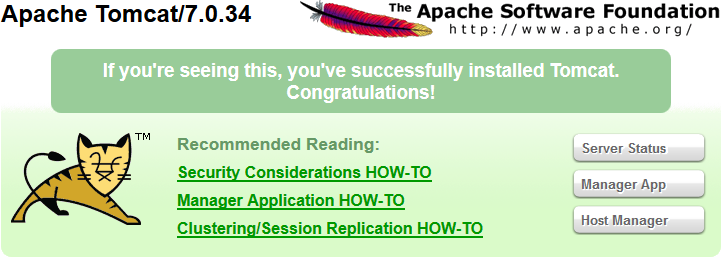
\includegraphics[scale=0.5]{img/setup/tomcat.png}
	\caption{Tomcat welcome screen}
	\label{fig:tomcat}
\end{figure}
\noindent
To deploy these applications, navigate to the following URL:
\begin{center}
	\texttt{http://<Your web server>:8080}
\end{center}
You should see something similar to Figure \ref{fig:tomcat}. Click on the button labelled "Manager App" and you will be prompted to enter your credentials. Use the username and password defined in the file \texttt{tomcat-users.xml}. The following page will show all the applications running on Tomcat right now. Below this table, there is a section called "Deploy" with subsection "WAR file to deploy". Simply select each of the two WAR files by clicking on the "Browse" button and then click on "Deploy". {\germinate} and {\gatekeeper} should now be listed in the applications table at the top of the page.

Clicking on the \texttt{Path} link in the first column of the overview table should redirect you to {\germinate} and {\gatekeeper} respectively.

\subsection{Running the {\germinate} Docker image}
If none of the previous options seem to be for you, we distribute our demonstration version of {\germinate} as a Docker image that you can run and try out yourself. This image is meant to be used as a first point of contact with {\germinate}. It allows you to run {\germinate} locally without having to install it. You can then explore the web interface and try out all the features that {\germinate} has to offer.

Detailed instructions for this Docker image are available online at:

\begin{center}
	\url{https://ics.hutton.ac.uk/germinate/germinate-docker-image/}
\end{center}

\subsection{Germinate Gatekeeper Admin}
\label{subsection:gatekeeper-admin}

\begin{figure}
	\centering
	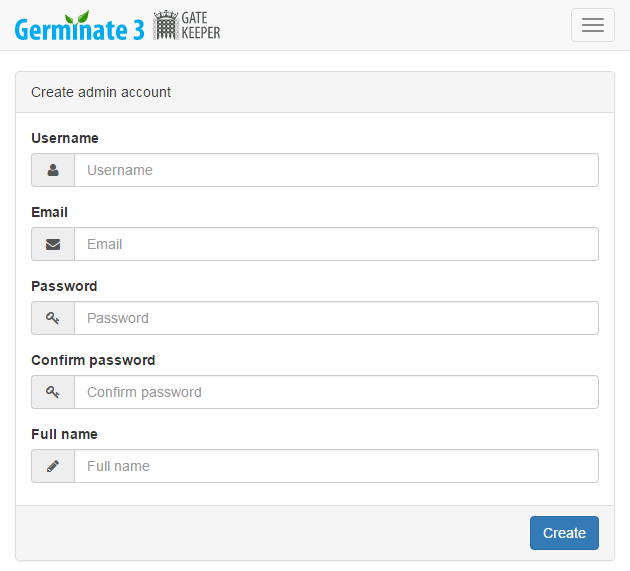
\includegraphics[scale=0.4]{img/setup/create-admin.png}
	\caption{Create admin account page}
	\label{fig:create-admin}
\end{figure}

The first time you go to the {\gatekeeper} website, you'll see the form shown in Figure \ref{fig:create-admin}. Fill it in to create the initial admin account. After this, you will be able to log in to Gatekeeper and create other users, database systems and set their permissions.

\subsection{Logging}
\label{subsection:logging}
Depending on your configuration (ref.\ \texttt{Germinate.Server.Logging.Enabled} in Section \ref{sec:config}), {\germinate} will log all server-side exceptions. This can be useful when you need to debug your version of {\germinate}.

The log files are stored to this location: \texttt{<Tomcat Directory>/temp/logs/}. Each instance of {\germinate} uses its own log files to avoid mix-ups.